\documentclass[../main.tex]{subfiles}
\begin{document}
	\subsection{Самосопряженные операторы. Изометрические операторы}
	\begin{defin}
		$\A \in End(V) \Space (V, (\cdot, \cdot)) \; \; \text{Унит. (евкл.)}$\n
		$\A$ называется \underline{самосопряженными}, если $\boxed{\A = \A^*}$\n
		т. е. $\forall x, y \in V \; \boxed{(\A x, y) = (x, \A y)}$\n
		Унит. пространство -- \underline{эрмитов} оператор\\
		Евклидово пространство -- \underline{симметричный} оператор\n
		Очевидно, $\A$ -- \underline{самосопр.}, то $\A$ -- \underline{нормальный}\\
		$\A \A^* = \A \A = \A^* \A$
	\end{defin}
	\textbf{Свойства:}
	\begin{mylist}
		\item $\A$ самосопр. $\Leftrightarrow \exists $ о.н.б., т.ч. $A = \vec{A^T} = A^* \begin{pmatrix}
			A\text{ -- эрмитова матрица (компл.)}\\
			A\text{ -- симм. матрица (вещ.)}
		\end{pmatrix}$
		\begin{proof}
			Свойство 1 (?) для сопряж. опер.\\
			$\forall $ о.н.б. $\begin{matrix}
				\A^* \leftrightarrow \A^* = \vec{A^T}\\
				\A \leftrightarrow A
			\end{matrix} \Leftrightarrow A = A^* = \vec{A^T}$
		\end{proof}
		\item 
		$\forall \A, \B$ самосопр. $\Rightarrow \underset{\text{самосопр. опер.}}{(\lambda \A + \B)} \; \; \forall \dunderline{\lambda \in \R}$ (упр.)
		\item $\left.\begin{array}{c}
			\forall \A, \B \text{ самосопр.}\\
			\A \circ \B = \underset{\text{перестанов.}}{\B \circ \A}
		\end{array}\right\} \Rightarrow \A \circ \B = \B \circ \A $ самосопр. (упр.)
		\item $\A$ самосопр. $\Leftrightarrow $\underline{все корни } характер. многочлена $\chi$ \underline{веществ.} (!)
		\begin{proof}\
			\begin{mylist}
				\item 
				$(V (\cdot, \cdot))$ \underline{унитарн.} $\A = \A^* \Rightarrow$ нормальн. $\Leftrightarrow \exists$ о.н.б., т.ч.\\
				матрица оператора $\A = $ \Space $\Lambda = diag(\lambda_1 \ldots \lambda_n) \; \; \lambda_i $ с.ч. $\A\n
				\A^* \leftrightarrow \vec \Lambda = diag (\vec \lambda_1 \ldots \vec \lambda_n)\n
				\A = \A^* \Leftrightarrow \Lambda = \vec \Lambda \Leftrightarrow \lambda_i = \vec{\lambda_i} = \Leftrightarrow \lambda_i \in \R$ с.ч. $\A \underset{\text{\underline{унит.}}}{\Leftrightarrow}$ все с.ч. $\lambda_i$ корни $\chi$
				\item 
				$(V, (\cdot, \cdot))$ \underline{евклид}. $\Space \A_\mathbb C$ продолж. $\A$ на $V_\mathbb C\n 
				\Rightarrow (\A_\mathbb C)^* = (\A^*)_\mathbb C \underset{\stackrel{\uparrow}{\A = \A^*}}{=} \A_\mathbb C \Rightarrow \A_\mathbb C$ самосопр. $\Leftrightarrow$ по п. а) Все корни $\chi_{\A_\mathbb C}$ вещ., $\chi_\A = \chi_{\A_\mathbb C} \Rightarrow \n \Rightarrow$ все корни $\chi_\A$ вещ.
 			\end{mylist}
		\end{proof}
		\item $\underset{\text{лин. подпр.}}{L} \subset V$ инвар. отн. $\A \Rightarrow L^\perp$ инвар. отн. $\A$
		\begin{proof}
			см. свойства сопряж. опер.
		\end{proof}
	\end{mylist}
	\begin{theorem}[Канонич. вид матрицы самосопряж. оператора]\ \\
		$\A \in End(V), \; \; V (\cdot , \cdot) $ унит. (евкл.)\n
		$\A$ самосопр. опер. $\Leftrightarrow \exists$ о.н.б. $V$ такой, что матрицы операторов $\A$ и $\A^*$ будут иметь в нем диагональынй вид $\Lambda = diag(\lambda_1 \ldots \lambda_n), \; \lambda_i \in \R$\n
		Очевидно, что базис состоит из о.н. с. в. $A\ (\A^*), \lambda_i \in \R$ соотв. с.ч. $\A\ (\A^*)$
	\end{theorem}
	\begin{proof}
		Т.к. $\A$ самосопр. $\Rightarrow \A$ норм. $\Rightarrow$ по теореме о кан. виде матрицы норм. опер.\n
		\underline{Унит:} $\A \leftrightarrow \Lambda = diag(\lambda_1 \ldots \lambda_n) \Space \lambda_i$ с.ч. $(\lambda_i \in \R \ \text{ св-во 4})$\n 
		\underline{Евкл:} $\A \leftrightarrow \Lambda = diag(\lambda_1 \ldots \lambda_n) \Space \lambda_i$ с.ч. $(\lambda_i \in \R \ \text{ св-во 4})$, блоков $\Phi_j$ не будет \n
		$\A = \A^*$ матрицы опер. совпад.
	\end{proof}
	\begin{corollary}
		$\A$ самосопр. опер. $\Leftrightarrow V = \bigoplus\limits_{\lambda \text{ с.ч.}} V_\lambda \; \; \begin{matrix}
			\forall \lambda \in \R\\
			V_\lambda \perp V_\mu \; \lambda \neq \mu
		\end{matrix} \Space V_\lambda$ собств. подпр.
	\end{corollary}
	\begin{corollary}
		$\forall$ симм. (эрмит.) матрицы $A \ (A = A^*)$\n
		$\exists$ ортог. (унит.) матрица $T \ (T^* = T^{-1})$, т.ч. \n
		$A$ \underline{симм.} ($A = A^T$): \Space $T^{-1} A T = T^T A T = \Lambda = diag(\lambda_1 \ldots \lambda_n)$\n
		\underline{$A$ эрмитова} ($A  = \vec{A^T}$): $\Space T^{-1} A T = \vec{T^T} A T = \Lambda = diag(\lambda_1 \ldots_n) \Sspace \lambda_i \in \R $ с.ч.$A$
	\end{corollary}
	\begin{proof}
		$T = T_{e\rightarrow v} \Space \begin{matrix}
			e \text{ -- канон. базис } \R^n (\mathbb C^n)\\
			v \text{ -- о.н.б. из с.в.}
		\end{matrix} \Rightarrow T \text{ ортог. (унит.)}$
	\end{proof}
	\begin{defin}
		\underline{Невырожденный} линейный оператор $Q \in End(V), \Space (V, (\cdot, \cdot))$ унит. (евкл.)\n
		называется \underline{изометрическим}, если $\boxed{Q^* = Q^{-1}}$, т.е. \n
		$\forall x, y \in V \; \; \boxed{(Q x, Q y) = (x, y)}$\n
		$((Q x, Q y)) = (x, \underbracket{Q^* Q}_\E y) = (x, y)$\n
		"Сохраняет расстояние и углы"\n
		\underline{унитар.} -- $Q$ \underline{унитарный} оператор\\
		\underline{евкл.} -- $Q$ \underline{ортогон.} оператор.
	\end{defin}
	Очевидно, что $Q$ \underline{изометрич.} $\Rightarrow Q$ нормальный: $Q Q^* = Q Q^{-1} = \E = Q^{-1} Q = Q^* Q$\n \\
	\textbf{Свойства изометр. оператора:}
	\begin{mylist}
		\item $Q$ изометр. $\Leftrightarrow \exists$ о.н.б. $\boxed{Q^{-1} = \vec{Q^T} = Q^*}$, где $Q$ матрица оператора $\Q$ в этом базисе\n
		(т.е. $Q$ унит. (компл.) ортог. (вещ.) матрица)
		\begin{proof}
			Свойство матрицы сопряж. опер. \n $\forall$ о.н.б. $Q^* = \vec{Q^T} = Q^{-1}$
		\end{proof}
		\item
		$\Q$ \underline{изометр.} $\Leftrightarrow \Q$ переводит о.н.б. в о.н.б.
		\begin{proof}
			$(\Rightarrow)$ $e$ о.н.б. $(e_i, e_j) = \delta_{ij}\\
			\pu v_i = \Q e_i \; \; i = 1 \ldots n\n
			(v_i, v_j) = (\Q e_i, \Q e_j) \underset{\text{изометр.}}{=} (e_i, e_j) = \delta_{ij} \Rightarrow v$ о.н.б\n
			$(\Leftarrow) e$ и $e'$ о.н.б. $V$, т.ч. $e'_i = \Q e_i$ \Space $\forall x, y \in V \Space x = \sum\limits_{i=1}^n x_i e_i \; \; y = \sum\limits_{y=1}^n y_j e_j\n
			(\Q x, \Q y) = \sum\limits_{i=1}^n \sum\limits_{j=1}^n x_i \vec y_j \; (\Q e_i, \Q e_j) = \sum\limits_{i=1}^n \sum\limits_{j=1}^n x_i \vec y_j \overset{=\delta_{ij}}{(e'_i, e'_j)} = \sum\limits_{i=1}^n x_i \vec y_i = (x, y) \Rightarrow \Q$ изометр.
		\end{proof}
		\item $\Q, R$ -- изометр. $\Rightarrow \Q \circ R$ изометр. (упр.)
		\item $\Q$ изометр. $\Rightarrow \Q^{-1}$ изометр. (упр.)
		\item $\boxed{\Q \text{ изометр.} \Leftrightarrow \text{ все корни } \chi \text{ по модулю равны 1}}$
		\begin{proof}\
			\begin{mylist}
				\item $(V, (\cdot, \cdot))$ унит. $\Space \Q^* = \Q^{-1} \Rightarrow \Q$ норм. опер. $\Leftrightarrow \exists$ о.н.б., т.ч. матрица $\Q$ имеет диагон. вид $\Lambda = (\lambda_1 \ldots \lambda_n) \Space \lambda_i$ с.ч. (все корни $\chi$)\n
				причем матрица $\Q^*  = \vec \Lambda = (\vec \lambda_1 \ldots \vec \lambda_n)\n
				\Q^* = \Q^{-1} \Leftrightarrow \vec \Lambda = \Lambda^{-1} \Leftrightarrow$ 
				$ \underbracket{\vec \Lambda \Lambda} = \underbracket{E}\n 
				\underbracket{\lambda_i \vec \lambda_i}_{|\lambda_i|^2} = 1 \Leftrightarrow |\lambda_i| = 1$
				\item $(V, (\cdot, \cdot))$ \underline{евклидово про-во}\n
				$\Q_\mathbb C$ продолж. $\Q$ на $V_\mathbb C \Space (\chi_{\Q_\mathbb C} = \chi_\Q)\n
				\Rightarrow (\Q_\mathbb C)^* = (\Q^*)_\mathbb C = (\Q^{-1})_\mathbb C\\
				(\Q^{-1})_\mathbb C = (\Q_\mathbb C)^{-1} \Sspace ?$ Можно ли переставить?\n
				$\Q$ невырожд. $\Leftrightarrow \underset{\neq 0}{det\ \Q} = \chi_\Q(0) = \chi_{\Q_\mathbb C}(0) = det\ \Q_\mathbb C \Leftrightarrow \Q_\mathbb C$ невырожд.\n
				Проверим, что $\Q_\mathbb C \cdot (Q^{-1})_ \mathbb C = \E \Space ?\n
				\forall x, y \in V \Space \Q_\mathbb C (\Q^{-1})_\mathbb C (x + iy) = \Q_\mathbb C (\underset{\text{вещ.}}{\Q^{-1} x} + i \underset{\text{вещ.}}{\Q^{-1} y}) = \n
				= \underbracket{\Q \Q^{-1}}_\E x + i \underbracket{\Q \Q^{-1}}_\E y = x + iy \Rightarrow (\Q_\mathbb C)^{-1} = (\Q^{-1})_\mathbb C$\\
				Аналогично: $(\Q^{-1})_\mathbb C \Q_\mathbb C = \E\n
				(\Q_\mathbb C)^* = (\Q_\mathbb C)^{-1} \Rightarrow \Q_\mathbb C$ изометр. на $V_ \mathbb C \Rightarrow$ по а) все корни $\chi$ по модулю $=1$
			\end{mylist}
		\end{proof}
	\begin{remark}
		$V$ евкл. $\Sspace \Q$ -- ортог. оператор $\Rightarrow $ все с.ч. $\Q = \pm 1$
	\end{remark}
	\item $\underset{\text{лин. подпр.}}{L} \subset V$ инвар. отн. $\Q \Rightarrow L^\perp$ инвар. отн. $\Q$
	\begin{proof}
		$\forall x \neq \0 \in L$, т.к. $\Q$ невырожд. $\Rightarrow \exists \underset{\neq \0}{z} \in L: x = \Q z\n
		\forall y \in L^\perp \; \; (x, \Q y) = (\Q z, \Q y) \underset{\text{изометр.}}{=} (\underset{\in L}{z} \underset{\in L^\perp}{y}) = 0 \Rightarrow \Q y \in L^\perp \Rightarrow L^\perp$ инвариант отн. $\Q$
	\end{proof}
	\end{mylist}
	\begin{theorem}[канонич. вид матрицы унитарного оператора]\ \\
		$(V, (\cdot, \cdot))$ \underline{унит.} $\Q \in End(V)$, \underline{невырожд.}\n
		$\Q$ унитарный оператор (изометр.) $\Leftrightarrow \exists$ о.н.б., т.ч. матрица оператора $\Q$ в этом базисе будет иметь диагональный вид: $\Lambda = diag(\lambda_1 \ldots \lambda_n)$, где $\lambda_j \in \mathbb C$ и $|\lambda_j| = 1 \; \; \forall j = 1\ldots n\n$
		при этом матрица $\Q^*$ будет иметь также диагон. вид: $\Lambda^{-1} = diag(1/\lambda_1 \ldots 1/\lambda_n) = \vec{\Lambda^T} = \Lambda^*$
	\end{theorem}
	\begin{proof}
		См. теорему о канон. виде матрицы норм. опер.\\
		$\Q$ унит. (норм. + все корни хар. мн. $\chi$ по модулю = 1) $\Leftrightarrow \exists$ о.н.б. матрица $\Q \; = \Lambda = diag(\lambda_1 \ldots \lambda_n)\n
		\lambda_i$ с.ч. $\Q$ (корни хар. мн-на) \n 
		$\forall i \; \lambda_i \neq 0$ (т.к. $\Q$ невырожд. $\overset{\neq 0}{det\ \Q} = \lambda_1 \cdot \ldots \cdot \lambda_n \cdot (-1)^n$) $\Space \underset{\text{т.к. } \Q \text{ унит.}}{\Lambda^* = \Lambda^{-1}} = diag(\frac{1}{\lambda_1} \ldots \frac{1}{\lambda_n})$
	\end{proof}
	\begin{corollary}
		$\Q$ унит. опер. $\Leftrightarrow V = \bigoplus\limits_{\lambda \text{с.ч.}} \underset{\text{собств. подпр.}}{V_\lambda} \; \; \; \lambda \in \mathbb C \; \; |\lambda| = 1 \; \; \Space V_\lambda \perp V_\mu \; \; \lambda \neq \mu$
	\end{corollary}
	\begin{corollary}
		$\forall$ унит. матрицы $Q\;  (Q^* = Q^{-1}) \; \; \exists$ унит. матрица $T\; (T^* = T^{-1})$\n
		т.ч. $T^{-1} Q T = \vec{T^T} Q T = \Lambda = diag(\lambda_1 \ldots \lambda_n)\n
		\text{ где } \lambda_i \in \mathbb C$ с.ч. $Q$, причем $|\lambda_i| = 1$\n 
		Все док-ва см. раньше (для самосопр., для норм.)
	\end{corollary}
	\begin{theorem}[Канонич. вид матрицы ортог. оператора]\ \\
		$(V, (\cdot, \cdot))$ \underline{евклидово} \Space $\Q \in End(V)$, \underline{невырожд.} \n
		$\Q$ ортог. оператор (изометр.) $\Leftrightarrow \exists$ о.н.б. $V$ такой, что матрица оператора $\Q$ в этом базисе будет иметь блочно-диагон. вид.\n
		$\Lambda = $ \belowbaseline[-24pt]{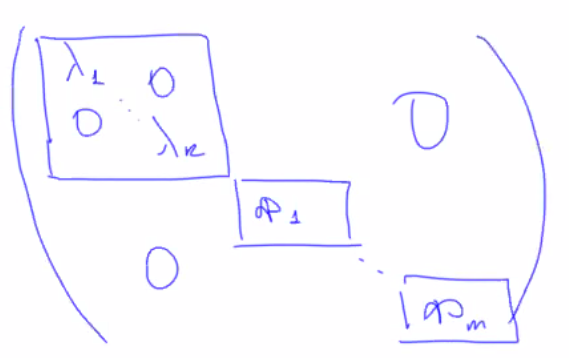
\includegraphics[width=150px]{pic100}}$\begin{matrix}
			\text{где } \lambda_i = \pm 1\n
			\Phi_j = \begin{pmatrix}
				\alpha_j & \beta_j\\
				\beta_j & \alpha_j
			\end{pmatrix} \; \begin{matrix}
				\alpha_j, \beta_j \in \R\\
				\alpha_j^2 + \beta_j^2 = 1
			\end{matrix}
		\end{matrix}\n$
		Причем, матрица оператора $\Q^*$ будет тоже иметь блочно диагон. вид\n
		$\Lambda^{-1} = \begin{pmatrix}
 			\begin{pmatrix}
				\lambda_1 & & 0\\
				& \ddots\\
				0 & & \lambda_k
			\end{pmatrix}\\
			& \begin{matrix}
				\boxed{\Phi^T_1} \\
				& \ddots\\
				& & \boxed{\Phi^T_m}
			\end{matrix}
		\end{pmatrix} = \Lambda^T \Space \Phi_j \Phi^T_j = E \; \; \; (\Phi_j^{-1} = \Phi^T_j)$
	\end{theorem}
	\begin{proof}
		см. теорему о канон. виде матрицы норм. опер. в евкл. про-ве\n
		$\Q$ ортог. $\Leftrightarrow \Q$ (нормал. + все корни хар. мн-на $\chi$ по модулю = 1) $\Leftrightarrow \n \Leftrightarrow
		\begin{matrix}
			\text{ с.ч. }\lambda_s = \pm 1 \n \text{компл. корни } |\alpha_j + i \beta_j | = \sqrt{\alpha_j^2 + \beta_j^2} = 1\end{matrix}$
		$\Rightarrow \Phi_j = \begin{pmatrix}
			\alpha_j & \beta_j\\
			-\beta_j & \alpha_j
		\end{pmatrix}$
	\end{proof}
	\begin{remark}
		$\Phi_j = \begin{pmatrix}
			\alpha_j & \beta_j\\
			-\beta_j & \alpha_j
		\end{pmatrix} \; \; \alpha^2_j + \beta^2_j = 1 \Space \alpha_j = \cos \phi \; \;  \beta_j = \sin \phi$\n
		$\begin{pmatrix}
			\cos \phi & \sin \phi \\
			-\sin \phi & \cos \phi
		\end{pmatrix} \leftrightarrow $
			поворот соотв. коорд пл-ти на угол \ $''-\phi''$\n 
		\begin{minipage}{0.4\textwidth}
			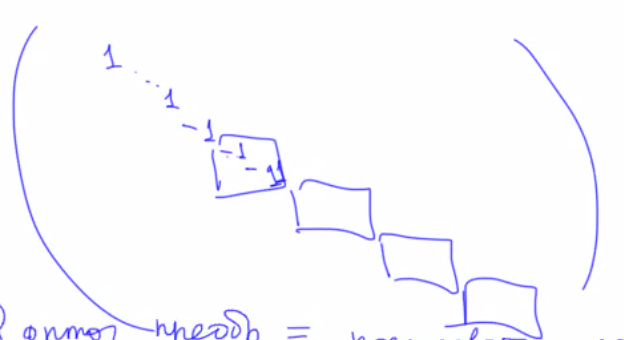
\includegraphics[width=\textwidth]{pic101}
		\end{minipage}
		\begin{minipage}{0.5\textwidth}
			$\boxed{\begin{matrix}
					-1 & 0 \\ 0 & -1
				\end{matrix}} \leftrightarrow$ поворот на угол $\pi$\n 
			$-1 \leftrightarrow$ "отражение" \ относительно соотв. \\ коорд. пл-ти
		\end{minipage}\n 
	$\Q$ ортог. преобразование $\equiv$ послеовательные повороты и отражения относительно коорд. осей
	\end{remark}
	\begin{corollary}
		$\forall$ \underline{ортог.} матрицы $Q \; (Q^T = Q^{-1})\n
		\exists$ ортог. матрица $T\; (T^T = T^{-1})$, т.ч.\\
		$T^{-1} Q T = T^T Q T = 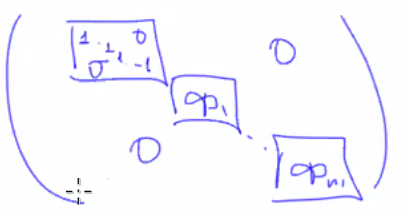
\includegraphics[width=130px]{pic102}$\n
		где $\pm 1$ с.ч. $Q$\n 
		$\Phi_j = \begin{pmatrix}
			\alpha_j & \beta_j \\
			-\beta_j & \alpha_j
		\end{pmatrix} \Space \begin{matrix}
			\alpha_j \pm i \beta_j \text{ компл. корни } \chi_\Q \\
			\alpha_j^2 + \beta_j^2 = 1
		\end{matrix}$
	\end{corollary}
	\subsection{Разложения матриц: $LU$, Холецкого, $QR$ и полярное}
	\begin{defin}\ \\
		$\underset{\text{'low'}}{L} = (l_{ij})_{n\times n} = 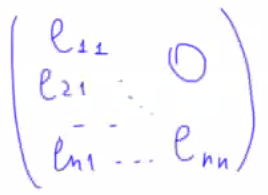
\includegraphics[width=100px]{pic103}$ называется \underline{нижняя (левая) треугольная матрица}\n
		Если $l_{ii} = 1 \; \forall i = 1\ldots n$, то добавляют \underline{унитреугольная}\n
		$\underset{\text{'up'}}{U} = (u_{ij})_{n\times n} = 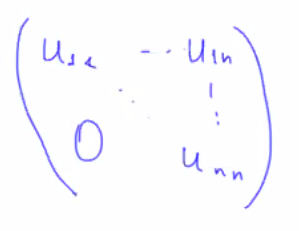
\includegraphics[width=100px]{pic104}$ называется \underline{верхняя (правая)} треуг. матрица.\n
		Если $u_{ii} = 1 \;\;  \forall i = 1\ldots n$, то добавляют \underline{унитреугольная}.
	\end{defin}
	\begin{defin}
		$A_{n\times n} = (A_{ij}) \; A_k = \begin{pmatrix}
			a_{11} & \ldots & a_{1k}\\
			&\ldots\\
			a_{k1} &\ldots &a_{kk}
		\end{pmatrix}$ \underline{угловая матрица}\n
		$\triangle_k = det A_k$ -- \underline{угловой минор } $A \Space \triangle_1 = a_{11} \Space \triangle_n = det A$
	\end{defin}
	\begin{theorem}[$LDU$ -- разложение $\;  A_{n\times n}$]\ \\
		$\forall k = 1\ldots n-1 \Space \triangle_k \neq 0 \Leftrightarrow$ \belowbaseline[-14pt]{
			$\begin{array}{l}
				\exists! L \text{ унитреугольная}\\
				\exists! U \text{ унитреуг.}\\
				\exists! D = diag(d_1 \ldots d_n), \; d_i \neq 0 \; \; i = 1 \ldots n-1 \n 
				\boxed{A = LDU}
		\end{array}$}\n 
	$A = \overset{\text{унитреуг.}}{\overset{\swarrow}{L} D \overset{\searrow}{U}}\Space = \Space
	\left.\begin{array}{l}
		\underset{\tilde{L} \text{ нижнетреуг.}}{\underbracket{LD} U} = \tilde L U\n 
		\underset{\tilde{U} \text{ верхнетреуг.}}{L\underbracket{DU}} = L \tilde U
	\end{array}\right\} $ -- $LU$ разложение (не единств. образом определяется)
	\end{theorem}
\end{document}